%; whizzy chapter
% -initex iniptex -latex platex -format platex -bibtex jbibtex -fmt fmt
% 以上 whizzytex を使用する場合の設定。

%     Kansai Debian Meeting resources
%     Copyright (C) 2007 Takaya Yamashita
%     Thank you for Tokyo Debian Meeting resources

%     This program is free software; you can redistribute it and/or modify
%     it under the terms of the GNU General Public License as published by
%     the Free Software Foundation; either version 2 of the License, or
%     (at your option) any later version.

%     This program is distributed in the hope that it will be useful,
%     but WITHOUT ANY WARRANTY; without even the implied warranty of
%     MERCHANTABILITY or FITNESS FOR A PARTICULAR PURPOSE.  See the
%     GNU General Public License for more details.

%     You should have received a copy of the GNU General Public License
%     along with this program; if not, write to the Free Software
%     Foundation, Inc., 51 Franklin St, Fifth Floor, Boston, MA  02110-1301 USA

%  preview (shell-command (concat "evince " (replace-regexp-in-string "tex$" "pdf"(buffer-file-name)) "&"))
% 画像ファイルを処理するためにはebbを利用してboundingboxを作成。
%(shell-command "cd image200708; ebb *.png")

%%ここからヘッダ開始。

\documentclass[mingoth,a4paper]{jsarticle}
\usepackage{kansaimonthlyreport}
\usepackage[dvips]{xy}
\usepackage{ascmac}

% 日付を定義する、毎月変わります。
\newcommand{\debmtgyear}{2010}
\newcommand{\debmtgdate}{22}
\newcommand{\debmtgmonth}{08}
\newcommand{\debmtgnumber}{38}

\begin{document}

\begin{titlepage}

% 毎月変更する部分、本文の末尾も修正することをわすれずに

 第\debmtgnumber{}回 関西 Debian 勉強会資料

\vspace{2cm}

\begin{center}
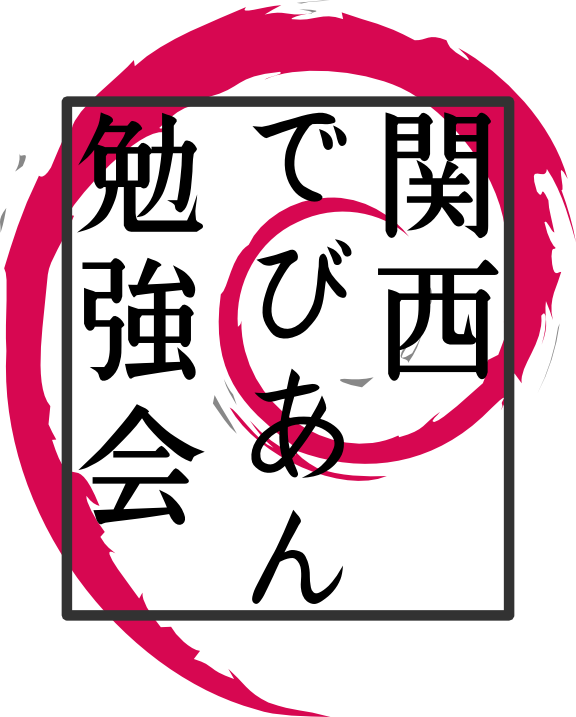
\includegraphics{image200802/kansaidebianlogo.png}
\end{center}

\begin{flushright}
\hfill{}関西 Debian 勉強会担当者 佐々木・倉敷・のがた \\
\hfill{}\debmtgyear{}年\debmtgmonth{}月\debmtgdate{}日
\end{flushright}

\thispagestyle{empty}
\end{titlepage}

\dancersection{Introduction}{Debian JP}

\subsection*{}%ロゴ用のスペース稼ぎ
 
関西 Debian 勉強会はDebian GNU/Linux のさまざまなトピック(新しいパッケー
ジ、Debian 特有の機能の仕組、Debian 界隈で起こった出来事、などなど)に
ついて話し合う会です。

目的として次の三つを考えています。
\begin{itemize}
      \item MLや掲示板ではなく、直接顔を合わせる事での情報交換の促進
      \item 定期的に集まれる場所
      \item 資料の作成
\end{itemize}

それでは、楽しい一時をお楽しみ下さい。

\clearpage

\begin{minipage}[b]{0.2\hsize}
 {\rotatebox{90}{\fontsize{80}{80}
{\gt 関西 Debian 勉強会}}}
\end{minipage}
\begin{minipage}[b]{0.8\hsize}
\hrule
\vspace{2mm}
\hrule
\setcounter{tocdepth}{1}
\tableofcontents
\vspace{2mm}
\hrule
\end{minipage}

\dancersection{最近のDebian関係のイベント報告}{Debian JP}

\subsection{DebConf10}

8 月 1 日$\sim$ 7 日に DebConf10 がアメリカ、ニューヨークで開催されました。
日本からはやまねさんや岩松さんが参加された模様です。
活発な議論/開発がなされた事でしょう。

今月の東京エリアDebian勉強会はお盆(?)で中止だったみたいなので、
今後の東京エリアDebian勉強会で DebConf10 の参加報告があるかと思います。

\subsection{Debian 6.0 ``squeeze'' frozen!!!!}

8 月 6 日(DebConf10期間中)に Debian 6.0 ``Squeeze'' のフリーズが
リリースチームより宣言されました%
\footnote{\url{http://www.debian.org/News/2010/20100806}}。
これによって unstable に存在するパッケージからの testing への自動的な移行が停止し、testing は frozen と呼ばれる状態になります。

squeeze での主なソフトウェアのバージョンは以下の通りです:
\begin{itemize}
      \item カーネル:
    \begin{itemize}
          \item Linux 2.6.32, 
        FreeBSD\footnote{7? 8?...詳細は杉本さんの発表を参照して下さい}
    \end{itemize}
      \item 
    デスクトップ環境:
    \begin{itemize}
          \item 
        X.org 7.5, KDE 4.4.5, Gnome 2.30.0, LXDE 0.5.0,  XFCE 4.6.2, 
        OpenOffice.org 3.2.1, ...
    \end{itemize}
      \item
    サーバ:
    \begin{itemize}
          \item 
        Apache 2.2.16, PHP 5.3.2, MySQL 5.1.48, PostgreSQL 8.4.4, Samba 3.4, 
        ...
    \end{itemize}
      \item
    プログラミング言語:
    \begin{itemize}
          \item Python 2.6 and 3.1, Perl 5.10, GHC 6.12 and GCC 4.4, ...
    \end{itemize}
\end{itemize}

とは言え、RC バグもまだまだ多いですし($\sim 850?$)、
RC とは言えなくても実用に耐えないバグの残ったパッケージに関しては
リリースチームに交渉することでパッケージを更新する事が可能です。

他にもインストーラ/移行マニュアルの翻訳更新作業など、
これからリリースに向けた作業が目白押しです。頑張りましょう。

\subsection{OSC 2010 Kansai@Kyoto}

前回の関西 Debian 勉強会は、OSC2010Kansai出展としての開催でした。
セッションは、
佐々木さんによる「野良ビルドから始めるDebianパッケージ作成」でした。
事前周知が間に合わずハンズオンとしては改善の余地がありましたが、
講義自体はウケもよく楽しんでもらえていたようでした。
%
急遽ミニセッションとして実施した GPG キーサインパーティも好評でした。
今後もOSCなどで実施していけるよう、水面下で動きがあるようです\footnote{%
コミュニティ横断的にキーサインパーティを開くための
ksp-ja MLが立ち上がりました。\url{http://groups.google.com/group/ksp-ja}}。

ブースでは機材の展示に加えて、「あんどきゅめんてっどでびあん」やDebian T
シャツ販売を行いました。また、オープンフォース徳島の河野由佳さんから
Debian の「ぐるぐるクッキー」の差し入れをいただきました。ありがとうござ
いました。

\begin{figure}[h]
    \centering
    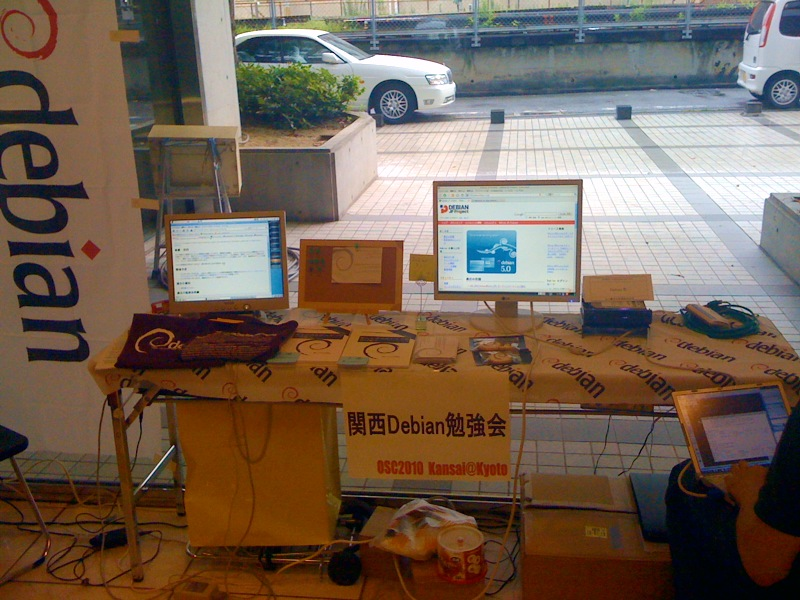
\includegraphics[width=0.49\textwidth]{image201008/osckyoto1.jpg}
    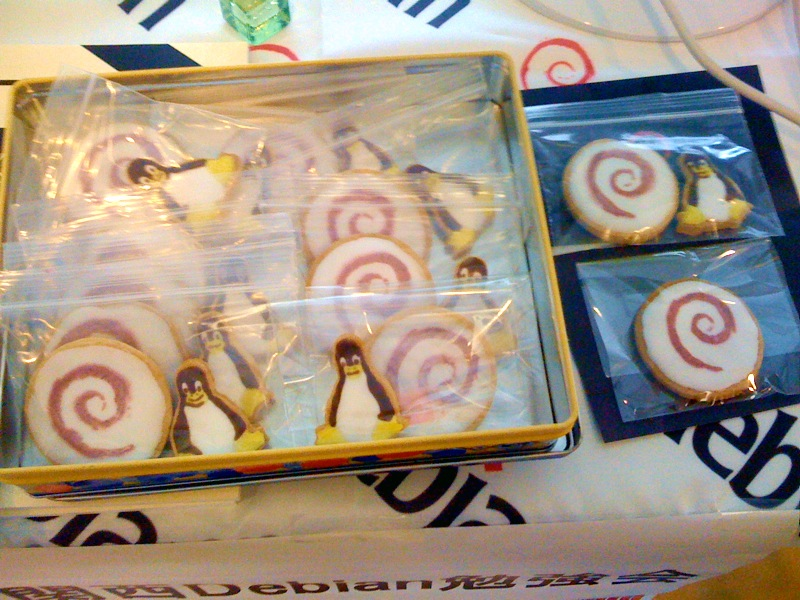
\includegraphics[width=0.49\textwidth]{image201008/osckyoto2.jpg}    
    \caption{(左)ブース展示と物販の様子. %
      (右)差し入れの Debian 「ぐるぐるクッキー」}
\end{figure}

\subsection{第 36 回関西 Debian 勉強会}

OSC の直前の6/27 にも、関西 Debian 勉強会が福島区民会館で開催されました。
この時は、久しぶりに ustream による中継も行われました。
%
セッション内容は、佐々木さんによる「debhelper7 と cdbs の深追い」と、
倉敷による「puppet に \$HOME を整理させよう」でした。

debhelper についてはあまり深追いできず消化不良な感が否めませんでしたが、
dh コマンドを使ったパッケージ作成の最初の一歩にはなったと思います。%
機会があれば応用編をやってみたいと思います。

puppet の方は、ハンズオンで puppet に親しんでもらう予定でしたがタイムオー
バーとなり、中途半端な終わり方になってしまいました。希望の有無に関わらず、
またいずれ puppet ネタを用意するつもりなので、その時は時間内におさまるよ
う精進します。

\dancersection{事前課題}{Debian JP}

今回は以下の課題を設定しました。
\begin{screen}
    \begin{enumerate}
          \item 
        Debian が動作する CPU、ターゲット機器について予習をしておいて下さい。
          \item 
        それらのうち、
        これまでに使用したことがあるアーキテクチャを教えてください。 \\
        (例:i386、amd64、arm、powerpcなど) 
          \item 
        組込み機器の OS として
        Debian を使う場合のメリット/デメリットについて、
        思う所を書いてください。 
    \end{enumerate}
\end{screen}

参加者の皆さんによる回答は以下の通りです。

\begin{prework}{ IPv6waterstar }
\begin{verbatim}
個人的には、arm以外のアーキテクチャでDebianをインストールもしくは使用したことがあります。一度、動いてしまえばどのアーキテクチャでもDeianである以上「不便」はありませんでした。
組込み機器のOSとしてDebianを使ってもいいと思うのですが、OSの基本的なレスポンスとして「遅い」のではないかと思います。
\end{verbatim}
\end{prework}

\begin{prework}{ 佐藤誠 }
\begin{verbatim}
1. http://www.debian.org/releases/stable/ 見てみました。
2. i386, amd64, powerpc
3. (たぶん)環境を早く整備できる。(ひょっとすると)痒いところに気づきにくいかもしれない。
\end{verbatim}

\end{prework}



\begin{prework}{ yabuki@netfort.gr.jp }

\begin{verbatim}
(1) 予習ということは、ハードを買ってハックせよと? ;-)
(2) i386,amd64,arm は所持している。さわったことがあるとか、sshしたとなるともうちょっと増えるけど。あとqemuでも作れますよね。環境は。
(3) メリット:Debianで得た有形無形の資産が、組込み機器でもつかえる。デメリット:組み込み機器は、Debianを使うことが目的ではなく、アプリケーションの動作をさせることが目的なので、Debianを使うことによるオーバヘッドが問題になるかどうか検討が必要だ。
\end{verbatim}

\end{prework}



\begin{prework}{ 古川竜雄 (frkwtto@gmail.com) }

\begin{verbatim}
1. これからします
2. i486とi686はあります
3. メリットはオープンソースとパッケージの多さ、ユーザーが多いことによる十分な情報。デメリットは商用利用? (知識がないので間違いかもしれません)
\end{verbatim}

\end{prework}



\begin{prework}{ 山田 洋平 }

\begin{verbatim}
2. Debian では i386 と amd64 だけですね。
3. ROM の関係で、apt-get が実機で使えないことと最小インストールに必要な容量が大きいことが解決できれば....
\end{verbatim}

\end{prework}



\begin{prework}{ dictoss(杉本 典充) }

\begin{verbatim}
1.予習しておきます。
2.i386、amd64、ppc(玄箱HG)、kfreebsd-i386、kfreebsd-amd64
3.メリットは、開発するものをドライバ・専用アプリに絞り込めるため開発量を減らせること、パッケージ形式になっているため不必要なファイルはアンインストールが容易であり小さいrootfsが作りやすいこと。
  デメリットはLinuxゆえにLinuxが動くハード性能が要求されること、開発したプログラムもDebianパッケージ化するはずなのでDebianパッケージについて知っている人にビルドの仕事が集中しそうなこと。
\end{verbatim}

\end{prework}


\begin{prework}{ 八津尾 雄介 }

\begin{verbatim}
2, i386, amd64, powerpc
3, 【メリット】アプリケーション・ミドルウェアが豊富, オープンソース
   【デメリット】起動・終了が遅い, リソースの大量消費
\end{verbatim}
\end{prework}



\begin{prework}{ SKINO }

\begin{verbatim}
2. i386、Alpha、UltraSparc(microSparc)
  その他、MIPSは悪戦苦闘中
3. 経験はございませんが、素人感覚的に
  メリット:
  ・サポートデバイスが豊富
  デメリット:
  ・パッケージの縛り
  ・カスタマイズは大変そう
\end{verbatim}

\end{prework}



\begin{prework}{ かわだてつたろう }

\begin{verbatim}
2. i386 と amd64 と sh4
3. 多くのパッケージ, セキュリティサポート, パッケージ管理システムが使用
 できることはメリットだとおもう。
\end{verbatim}

\end{prework}



\begin{prework}{ のがたじゅん }

\begin{verbatim}
1. はい。
2. 実際に使ったことがあるのはi386とamd64だけです。Digoo A320というゲーム機やNano NoteがJZ4740というmipsアーキテキクチャマシンなので、いじりたいなと思いつつそのまま放置になっています。
3. メリットは使い慣れたDebianの環境で使えることでしょうか。デメリットは、それを感じるぐらいまで使ったことがないのでよくわかりません。
\end{verbatim}

\end{prework}



\begin{prework}{ 山下康成 }

\begin{verbatim}
1. (予習って何をすればいいのでしょう)
2. arm, armel
3. 広いアーキテクチャをサポートしていて、第三世代LinkStation ではDebian GNU/Linux 以外の選択肢はありませんでした。
カーネルさえ動けばあとは Debian の豊富なパッケージがそのまま(ちょっと言いすぎ)利用させていただけるので、苦労なく Debian 化させていただくことが可能でした。
組込みでは X を使うことが少ないのに X 関連パッケージに依存するパッケージが多く、実質不要なパッケージまでインストールしなければならないのがデメリットでしょうか。
\end{verbatim}

\end{prework}



\begin{prework}{ ”まさ”こと”甲斐正三”です }

\begin{verbatim}
1. Debian が動作する CPU、ターゲット機器について予習をしておいて下さい。
 
   (1) Debian正式サポートCPU:
       [alpha][amd64][arm][armel][hppa][i386][ia64][mips][mipsel][powerpc][sparc]
   (2) Debianがサポートする訳ではないが、Debianの走るCPU:
       [m68k][SH3/4]
   (3) Debianがサポートするターゲット機器
       わかりません。
 
2. それらのうち、これまでに使用したことがあるアーキテクチャを教えてください。(例:i386、amd64、arm、powerpcなど)
    [armel]    armadillo9、ワンボード。 debianです。
    [i386]     msi,intelマザーボードの手作りPC
    [powerpc]  iMac(ボンダイブルー)、'linux for ppc'です。その当時DebianにPPCがあることを知りませんでした。
    [SH3]      T-SH7706LAN rev.2.0 SH3 w/LAN/SD ボード、Debianではありません。
 
3. 組込み機器の OS として Debian を使う場合のメリット/デメリットについて、思う所を書いてください。
    組込みOSを云々できるほど経験がありませんが、
    希望としては、
      ・開発環境の構築が簡単にできる。(DebianでサポートされていないCPUであっても)
      ・きめ細かいインストールが可能。
      ・ブートも含めて組込みに関するドキュメントが豊富。
    などです。
以上。
\end{verbatim}


\end{prework}

\begin{prework}{  清野陽一 }

\begin{verbatim}
1.はーい
2.i386,amd64,ppc,arm
3.余計なパッケージを入れずに済むこと…かなぁ…。
\end{verbatim}

\end{prework}

\begin{prework}{ lurdan }

\begin{verbatim}
2. i386 (常用), amd64 (常用),  arm (Zaurus), sh4 (リビルドごっこ), powerpc (玄箱、初代TeraStation), alpha (入れただけ), kfreebsd-amd64 (ビルドテスト用)
3. メリット:組み込み Linux (のディストリビューション) としては事例が豊富っぽいのと、ユニバーサルオペレーティングシステムとしての debian 自体が eglibc や emdebian などで組み込みを意識しているあたり、後は最低限動作に必要な構成を作るのが超簡単とか。組み込み向け skkserv もあるよ!
   デメリット:日本の組み込み業界的には、メーカーからポンとドキュメントもらえた方が嬉しそう。
\end{verbatim}

\end{prework}

\begin{prework}{ 坂本 敏久(サカモト トシヒサ) }

\begin{verbatim}
はじめまして、坂本といいます。
2週間前にDebianを使いはじめた初心者です。
(ちなみにLinuxもほぼ初心者です。)
よろしく、お願いします。

今回の課題は、無回答でお願いします。
\end{verbatim}

\end{prework}

\dancersection{Debian GNU/kFreeBSDで暮らせる環境を構築してみる。}{杉本 典充}

\subsection{Debian GNU/kFreeBSDについて}

\subsubsection{Debian GNU/kFreeBSDとは}
「Debian GNU/kFreeBSD」とはカーネルにFreeBSDカーネル、ユーザランドにDebianの
ポリシーやパッケージシステムを取り入れたOSです。
Debian ProjectはLinuxカーネル以外のカーネルを用いたOSを作成する取り組みも
行っており\footnote{\url{http://www.debian.org/ports/}}、
Debian GNU/kFreeBSDはSqueezeでのリリースを目指して開発が進んでいます。


Debian GNU/kFreeBSDはi386版とamd64版のアーキテクチャが利用できます。

Debian GNU/kFreeBSDについては以下に情報が公開されています。

\begin{itemize}
 \item Debian Wiki      : \url{http://wiki.debian.org/Debian\_GNU/kFreeBSD}
 \item Debian Wiki(FAQ) : \url{http://wiki.debian.org/Debian\_GNU/kFreeBSD\_FAQ}
 \item Mailing List     : \url{http://lists.debian.org/debian-bsd/}
 \item IRC              : \#debian-kbsd at irc.debian.org
\end{itemize}

\subsubsection{Debian GNU/kFreeBSDとDebian GNU/Linuxの違い}
Debian GNU/kFreeBSDから見たDebian GNU/Linuxとの違いについて以下に一例を
上げます。

\begin{itemize}
 \item デバイスドライバはFreeBSDの流儀に従う。
 \begin{itemize}
  \item サウンドデバイスはOSSを利用する。
  \item ネットワークデバイス名が「eth0」等の固定名ではなくネットワークドライバによって変わる。
  \item ディスクデバイス名が「/dev/ad4s1」のような形式になる。
  \item mountコマンドのオプションが若干異なる。(USBメモリで利用されるFAT32はvfatではなくmsdosfsを用いる。)
 \end{itemize}
 \item ファイルシステムは(FreeBSDで実装している)UFS、ext2\footnote{Debian GNU/kFreeBSDでext3は読み込みのみサポート。\url{http://wiki.debian.org/Debian_GNU/kFreeBSD_FAQ}}が使える。
\footnote{ZFSはユーザランドツールが未整備のためまだ利用できない。}
 \item 仮想化はFreeBSD Jail、VirtualBox、qemuを使う。(KVMはLinux特有の機能のため使えない。他のOSを動かしたい場合はDebian GNU/kFreeBSDは不利。)
\end{itemize}

その他のaptによるパッケージシステムやディレクトリ構造はDebian GNU/kFreeBSDも
Debian GNU/Linuxも同じため、Debian GNU/Linuxの利用者であればすぐに慣れます。

\subsection{Debian GNU/kFreeBSDのインストール}

Debian GNU/kFreeBSDのインストーラはdailyビルドのイメージがありますので、
以下からダウンロードします。

\begin{itemize}
 \item i386  : \url{http://d-i.debian.org/daily-images/kfreebsd-i386/}
 \item amd64 : \url{http://d-i.debian.org/daily-images/kfreebsd-amd64/}
\end{itemize}

今回使用したインストーラはi386版の2010年6月19日のビルドを利用しました。
\footnote{インストーラは当たり外れがあるようで、ディスクのパーティションを作成する処理が正常に動作せず
インストール処理を進めることができないビルドが多かったです。そのため、パーティション作成に失敗する
ビルドは諦めて、ビルド時期が少し前のビルドを使用して再チャレンジすることを
おすすめします。}

インストールCDを作成し、PCにCDをセットして起動するとインストーラが起動します。

\begin{figure}[H]
\begin{center}
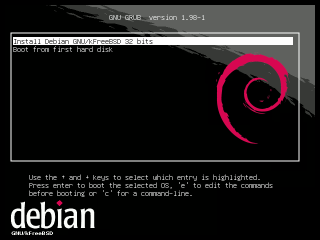
\includegraphics{image201008/kfreebsd-installer.png}
\caption{Debian GNU/kFreeBSDのDebianインストーラ}\label{debinstaller}
\end{center}
\end{figure}

インストール中の設定は以下を指定してインストールしました。

\begin{itemize}
 \item localeは「C」。(現時点のインストーラでは「C」と「English」のみの
localeしか指定できないため。)
 \item タイムゾーンはAsia/Japan。
 \item インストールは「Standard system utilities」(=Base System)のみ。
\end{itemize}

\subsection{初回起動}
\subsubsection{前準備}
X Window Systemをインストールしていないため、再起動後はコンソール環境で
起動します。
起動時にDHCPクライアントが起動するため、有線LAN環境であればIPアドレスを自動で
取得してネットワークにつながります。(以前は手動でdhclientを起動しないと
つながらなかった。)

カーネル起動後にインストーラで作成したユーザでログインし、最低限必要な以下の
パッケージをインストールし設定します。

\begin{commandline}
$ su
# apt-get update
# apt-get install sudo vim
# visudo
\end{commandline}

\subsubsection{カーネルの更新}

カーネルの起動メッセージを眺めているとCPUが1つしか認識していないように見えます。
現在起動中のカーネルとCPUの認識数を確認するとやはり1つしか認識していません。

\begin{commandline}
$ uname -a

GNU/kFreeBSD deb-NorTP60 7.3-1-686 #0
Tue Jul 20 02:12:21 CEST 2010 i686 i386
Genuine Intel(R) CPU           T2400  @ 1.83GHz GNU/kFreeBSD
\end{commandline}

\begin{commandline}
$ cat /proc/cpuinfo

processor   : 0
vendor_id   : GenuineIntel
cpu family  : 6
model       : 7
model name  : Genuine Intel(R) CPU           T2400  @ 1.83GHz
stepping    : 8
flags       : fpu vme de pse tsc msr pae mce cx8 apic sep mtrr pge mca
              cmov pat b19 b21 mmxext mmx fxsr xmm b26 b27 b28 b29 3dnow
cpu MHz     : 1828.76
bogomips    : 1828.76
\end{commandline}

現在利用できるカーネルを検索すると以下の候補が出てきます。

\begin{commandline}
$ apt-cache search kfreebsd-image-*

kfreebsd-headers-7.3-1-486 - header files for kernel of FreeBSD 7.3
kfreebsd-headers-7.3-1-686-smp - header files for kernel of FreeBSD 7.3
kfreebsd-headers-7.3-1-686 - header files for kernel of FreeBSD 7.3
kfreebsd-image-7-486 - kernel of FreeBSD 7 image
kfreebsd-image-7-686-smp - kernel of FreeBSD 7 image
kfreebsd-image-7-686 - kernel of FreeBSD 7 image
kfreebsd-image-7.3-1-486 - kernel of FreeBSD 7.3 image
kfreebsd-image-7.3-1-686-smp - kernel of FreeBSD 7.3 image
kfreebsd-image-7.3-1-686 - kernel of FreeBSD 7.3 image
kfreebsd-headers-8.0-1-486 - header files for kernel of FreeBSD 8.0
kfreebsd-headers-8.0-1-686-smp - header files for kernel of FreeBSD 8.0
kfreebsd-headers-8.0-1-686 - header files for kernel of FreeBSD 8.0
kfreebsd-image-8-486 - kernel of FreeBSD 8 image
kfreebsd-image-8-686-smp - kernel of FreeBSD 8 image
kfreebsd-image-8-686 - kernel of FreeBSD 8 image
kfreebsd-image-8.0-1-486 - kernel of FreeBSD 8.0 image
kfreebsd-image-8.0-1-686-smp - kernel of FreeBSD 8.0 image
kfreebsd-image-8.0-1-686 - kernel of FreeBSD 8.0 
\end{commandline}

シングルプロセッサ用とマルチプロセッサ用のカーネルは別々のようですので
マルチプロセッサ用カーネルをインストールし、再起動します。
\footnote{HyperThreadingのセキュリティ上の脆弱性に対応するためFreeBSD本家が
リリースするカーネルはHyperThreadingがデフォルトでOFFになっています。
Debian GNU/kFreeBSDでデフォルトがOFFであるかは対応CPUを持っていないため
確認できていません。}

カーネルのインストール処理でgrub2もアップデートされます。
\footnote{kfreebsd-image-8.0-1-686-smpをインストールしてみましたが、
インストール後に/へパーティションをマウントする処理に失敗し
起動できませんでした。FreeBSD 8.0 Release Noteに「''dangerously dedicated'' mode for the UFS file system is no longer supported. Important: Such disks will need to be reformatted to work with this release.」
という記述があるため、7.3から8.0へのカーネルアップグレードは
少し難しいようです。}

\begin{commandline}
$ sudo apt-get install kfreebsd-image-7.3-1-686-smp
$ sudo reboot
\end{commandline}

再起動し、カーネルとCPUの認識数を確認します。

\begin{commandline}
$ uname -a

GNU/kFreeBSD deb-NorTP60 7.3-1-686-smp #0
Tue Jul 20 02:43:20 CEST 2010 i686 i386
Genuine Intel(R) CPU           T2400  @ 1.83GHz GNU/kFreeBSD
\end{commandline}

\begin{commandline}
$ cat /proc/cpuinfo

processor   : 0
vendor_id   : GenuineIntel
cpu family  : 6
model       : 7
model name  : Genuine Intel(R) CPU           T2400  @ 1.83GHz
stepping    : 8
processor   : 1
vendor_id   : GenuineIntel
cpu family  : 6
model       : 7
model name  : Genuine Intel(R) CPU           T2400  @ 1.83GHz
stepping    : 8
flags       : fpu vme de pse tsc msr pae mce cx8 apic sep mtrr pge mca
              cmov pat b19 b21 mmxext mmx fxsr xmm b26 b27 b28 b29 3dnow
cpu MHz     : 1828.76
bogomips    : 1828.76
\end{commandline}

\subsection{Xorgのインストール}
X Window System環境が日常を過ごすため、xorgをインストールします。
しかしパッケージのインストール処理で以下のエラーが発生し、途中でインストールが
停止しました。

\begin{commandline}
$ sudo apt-get install xorg
Setting up hal (0.5.14-3) ...
Reloading system message bus config...
Failed to open connection to "system" message bus:
Failed to connect to socket /var/run/dbus/system_bus_socket: Connection refused
invoke-rc.d: initscript dbus, action "force-reload" failed.
Starting Hardware abstraction layer: haldinvoke-rc.d: initscript hal,
action "start" failed.
dpkg: error processing hal (--configure):
 subprocess installed post-installation script returned error exit status 1
\end{commandline}

\subsubsection{対応}

上記はhalのインストールの後処理でdbusの設定を再読み込みしようとしてエラーが
発生したため、パッケージのインストールが停止しました。
\footnote{\url{http://bugs.debian.org/cgi-bin/bugreport.cgi?bug=469528}}

psコマンドでdbusプロセスがいるか確認すると存在しません。
バグ修正はまだ行われていないため、とりあえずの措置として
「{\$} sudo /etc/init.d/dbus start」を実行してdbusを起動し
再度「{\$} sudo apt-get install xorg」を試みると次は以下のエラーに
変わりました。

\begin{commandline}
$ sudo /etc/init.d/dbus start
$ sudo apt-get install xorg
Setting up xserver-xorg (1:7.5+6) ...
invoke-rc.d: initscript hal, action "restart" failed.
dpkg: error processing xserver-xorg (--configure):
subprocess installed post-installation script returned error exit status 1
\end{commandline}

今度はxserver-xorgのインストールの後処理でhalと同様のエラーが発生したため、
再度halと同様に以下コマンドを実行し、xorgのインストールは完了しました。

\begin{commandline}
$ sudo /etc/init.d/dbus start
$ sudo apt-get install xorg
\end{commandline}

\subsubsection{X Window System起動及び設定}

この状態でstartxコマンドを実行するとX Window Systemの起動に成功しました。
しかし「/etc/X11/xorg.conf」の設定を確認しようとするとファイル自体が
存在しないためxorg.confを手動で作成します。

\begin{commandline}
$ sudo X -config
$ sudo cp xorg.conf.new /etc/X11/xorg.conf
\end{commandline}

再度startxを実行し、作成したxorg.confを用いてX Window Systemの起動が
確認できました。「/var/log/Xorg.0.log」を確認し'(EE)'の部分はないため、
動作は正常です。

\subsubsection{gdmのインストール(断念)}

ログイン画面もGUIで行いたいのでgdmをインストールします。

\begin{commandline}
$ sudo apt-get install gdm
\end{commandline}

gdmをインストールしrebootせずにgdmコマンドを実行するとマウス、キーボードは
問題なく動作します。

reboot後、自動でgdmが起動するのですがgdmのログイン画面でマウスは動きますが
キーボードが動作しません。(USBキーボードも動作しなかった。)

不本意ながらgdmによるログインは諦めstartxによる X Window Systemの起動に
切り替えることにしました。しかしこの状態ではカーネルの起動直後にgdmが
勝手に起動しキーボード入力ができなくなるため仮想コンソールに切り替えることも
できす、gdmをpurgeできません。

そのため、一度電源スイッチを長押ししてPCを停止、再起動してgdmが起動する前に
「Ctrl + Alt + F1」を連打してなんとか仮想コンソールに入り以下を実行してgdmを
purgeしました。

\begin{commandline}
$ sudo apt-get purge gdm
\end{commandline}

\subsection{デスクトップ環境の構築}

統合デスクトップ環境である「Xfce4」をインストールし、startxでXfce4を
起動するように.xinitrcを記述します。
.xinitrcは実行権が必要なため、実行権を付与します。

\begin{commandline}
$ sudo apt-get xfce4 xfce4-goodies
$ vim ~/.xinitrc
exec xfce4-session

$ chmod 744 ~/.xinitrc
$ startx
\end{commandline}

\subsection{日本語環境}

\subsubsection{日本語の表示}

日本語フォントをインストールします。

\begin{commandline}
$ sudo apt-get otf-ipafont otf-ipaexfont
\end{commandline}

日本語環境の「ja\_JP.UTF-8」ロケールはインストールされていなかったため
追加インストールします。

\begin{commandline}
$ sudo apt-get locales-all
\end{commandline}

startxコマンドでX Window Systemを起動するためlocaleの設定を.xinitrcに追記します。
Xfce4を終了して再度startxコマンドを実行するとXfce4が日本語環境で起動します。

\begin{commandline}
$ vim ~/.xinitrc    

export LANGUAGE='ja_JP.UTF-8'
export LC_ALL='ja_JP.UTF-8'
export LANG='ja_JP.UTF-8'
exec xfce4-session

$ startx
\end{commandline}

\subsubsection{日本語入力}

日本語入力環境としてuimを使用したいため、uimのインストールと設定をします。

\begin{commandline}
$ sudo apt-get install uim uim-anthy
$ vim ~/.xinitrc

export LANGUAGE='ja_JP.UTF-8'
export LC_ALL='ja_JP.UTF-8'
export LANG='ja_JP.UTF-8'

export XMODIFIRES='@im=uim'
export GTK_IM_MODULE='uim'
export QT_IM_MODULE='uim'

exec xfce4-session

$ startx
\end{commandline}

\subsection{開発環境のインストール}

Debian GNU/kFreeBSDのデバッグに必要なコンパイラ、パッケージの作成ツールを
インストールします。

\begin{commandline}
$ sudo apt-get update
$ sudo apt-get install gcc g++ gdb make
$ sudo apt-get install build-essential pbuilder debian-keyring
\end{commandline}

debパッケージのビルドができるかtcshをビルドして確認します。

\begin{commandline}
$ apt-get source tcsh
$ sudo apt-get build-dep tcsh
$ cd tcsh-6.17.00
$ dch
$ debuild -i -us -uc -b
$ sudo dpkg -i tcsh_6.17.00-3.1_kfreebsd-i386.deb
\end{commandline}

\subsection{Debian勉強会資料のビルド環境}

Debian勉強会での原稿はtexを採用しているため、原稿ファイルのビルド環境を
構築します。

texのビルドにはconrtib、non-freeのパッケージが必要なため、
apt-lineを修正します。

\begin{commandline}
$ sudo vim /etc/apt/sources.list
# deb http://ftp.jp.debian.org/debian/ squeeze main

deb http://ftp.jp.debian.org/debian/ squeeze main contrib non-free
deb-src http://ftp.jp.debian.org/debian/ squeeze main contrib non-free

deb http://security.debian.org/ squeeze/updates main
deb-src http://security.debian.org/ squeeze/updates main
\end{commandline}

必要なパッケージをインストールします。

\begin{commandline}
$ sudo apt-get install git-core
$ sudo apt-get install gs gs-esp gs-cjk-resource
$ sudo apt-get install ptex-bin xdvik-ja dvipsk-ja
$ sudo apt-get install okumura-clsfiles vfdata-morisawa5
$ sudo apt-get install texlive-latex-extra
$ sudo apt-get install poppler-data
$ sudo apt-get install evince
\end{commandline}

資料をダウンロードし、ビルドします。

\begin{commandline}
$ cd
$ git clone git://git.debian.org/git/tokyodebian/monthly-report.git/
$ cd monthly-report
$ make
\end{commandline}

\subsection{その他の日常環境の構築}

その他のよく使うソフトをインストールします。

\begin{commandline}
$ sudo apt-get install emacs emacs23-el
$ sudo apt-get install sylpheed sylpheed-i18n
$ sudo apt-get install iceweasel iceweasel-l10n-ja
$ sudo apt-get install audacious audacity
$ sudo apt-get install gxine
$ sudo apt-get install jd
$ sudo apt-get install gftp
\end{commandline}

\subsection{デバイスドライバ}
audaciousは音楽再生ソフトなのですが、実行しても音が鳴りません。
サウンドドライバをロードしているか確認するため「kldstat」を実行します。
\footnote{FreeBSDカーネルで読み込み中のカーネルモジュールの一覧を出力する
コマンドはkldstatですが、Debian GNU/KFreeBSDではlsmodがkldstatのリンクに
なっているためlsmodでも一覧を出力できます。}

\begin{commandline}
$ kldstat
 1   10 0xc0400000 890000   kfreebsd-7.3-1-686-smp.gz
 2    1 0xc0d9c000 57fdc    acpi.ko
 3    1 0xc5c7a000 67000    radeon.ko
 4    1 0xc5ce1000 14000    drm.ko
\end{commandline}

サウンドドライバがロードされていないためロードします。
\footnote{snd\_hdaはIntel945チップセットで音を鳴らすために必要な
サウンドドライバです。異なるサウンドチップを利用している場合は
環境に合わせてロードしてください。}

\begin{commandline}
$ sudo kldload snd_hda
$ kldstat
 1   10 0xc0400000 890000   kfreebsd-7.3-1-686-smp.gz
 2    1 0xc0d9c000 57fdc    acpi.ko
 3    1 0xc5c7a000 67000    radeon.ko
 4    1 0xc5ce1000 14000    drm.ko
 5    1 0xc611f000 1a000    snd_hda.ko
 6    1 0xc6139000 40000    sound.ko
\end{commandline}

音が鳴ることは確認できましたが、再起動するとサウンドドライバが読み込まれて
いない状態になります。そのため「/etc/modules」ファイルにカーネル起動時に
自動で読み込むドライバを設定します。
\footnote{Debian GNU/kFreeBSDに/sbin/modprobeコマンドはあるのですが
/sbin/kldloadのリンクになっているため、modprobeをしただけで再起動後も
自動でモジュールを読み込むようにはなっていないようです。}

\begin{commandline}
$ sudo vim /etc/modules
# /etc/modules: kernel modules to load at boot time.
#
# This file should contain the names of kernel modules that are
# to be loaded at boot time, one per line.  Comments begin with
# a ``#'', and everything on the line after them is ignored.
snd_hda.ko
\end{commandline}

\subsection{今後の課題}
Debian GNU/kFreeBSDでセットアップ作業を行いましたが日常生活を送るに向けて
いくつか課題が残っています。

\begin{itemize}
 \item WebブラウザでのFlashの再生(Adobe公式のFlashバイナリにFreeBSD版は
まだない)
 \item ビデオ再生(映像が乱れる。おそらくcodecの問題)
\end{itemize}

今後にむけた取り組みとして以下を試していきたいです。

\begin{itemize}
 \item Linuxバイナリ互換機能
 \item 仮想化機能(Jail、VirtualBox、qemu)
 \item ZFS
\end{itemize}

\subsection{環境構築を終えて}
インストーラの整備も進んでおり、X Window Systemの導入後はDebian GNU/Linuxと
なんら変わらない手順で環境構築ができました。

ただ問題が発生したときにFreeBSDカーネルとDebianの両方の知識が必要なため、
原因を調べるのが大変でFreeBSDとDebianの両方の情報源に当たってなんとか
解決しました。

バグ報告があると同じところでつまずいている人と情報を共有できるので
できるだけバグ報告は上げましょう。

Debian GNU/kFreeBSDは品質も徐々に上がってきており、Squeezeで技術プレビュー
扱いのリリースがされる予定です。\footnote{\url{http://www.debian.org/News/2010/20100806}}
みなさんもぜひDebian GNU/kFreeBSDをデバッグしてSqueezeリリースまでに品質を
高めましょう。

\subsection{参考資料}
\begin{itemize}
 \item 東京エリア Debian 出張勉強会 発表スライド(岩松信洋) : \url{http://tokyodebian.alioth.debian.org/pdf/debianmeetingresume201006-iwamatsu-presentation.pdf}
 \item Debian wiki : \url{http://wiki.debian.org/Debian\_GNU/kFreeBSD\_FAQ}
\end{itemize}

\dancersection{Emdebian について -関西 Debian 勉強会参加者中間報告- }{たなかとしひさ}

\subsection{前書き}

この資料は、筆者が Emdebian を使う上で勉強した事を記載しています。まだま
だ、完全に理解したわけではなく、部分部分でしかEmdebianを使えていませんが、
中間報告と言う事でご容赦ください。

\subsection{Emdebian って?}

Emdebian (Embedded Debian)は、Debian GNU/Linuxを元に、組込み機器用途に最
適化していくプロジェクトです。

Debian GNU/Linux は、まず Debian自身がマルチアーキテクチャ(勉強会課題1)に
対応しています。また、どのベンダーからも独立しており、Debian 社会契約、お
よび膨大な利用可能ソフトウェアは様々な選択肢を可能にしますが、デスクトッ
プ環境(大きなハードディスクとメモリ)に向けられています。

`Embedded Debian`は、Debian のメリットを活かしつつ、組込み機器の様な小さ
いシステム向けに Debian を軽量にするものです。

(上記は、\url{http://www.emdebian.org/}から意訳したものです)

\subsubsection{勉強会課題1: Debian が動作する CPU、ターゲット機器}

\url{http://www.jp.debian.org/ports/}から、Debian の移植版に関する情報が
得られます。

\begin{itemize}
 
 \item Intel x86 / IA-32 (i386) - 1番身近で使われていますね。 
 \item (Motorola 68k (m68k)) - Etch 以降のリリースには含まれていません。
 \item  Sun SPARC (sparc)

 \item  Alpha (alpha)
 \item  Motorola/IBM PowerPC (powerpc)
 \item  ARM (arm および armel) - 今回取り上げる CPU です。
 \item  MIPS CPUs (mipsとmipsel)
 \item  HP PA-RISC (hppa)
 \item  IA-64 (ia64)
 \item  S/390 (s390)
 \item  AMD64 (amd64)
\end{itemize}

Debianは、カーネルにLinuxカーネルを使いますが、Debian GNU/kFreeBSDの様に、
カーネルにFreeBSDのカーネルを使うものもあります。

\subsubsection{勉強会課題2: 皆さん、上記の内、使った事のあるアーキテクチャを教えてください。}

なお、Emdebian は、下記のアーキテクチャが利用可能です。

i386、amd64、powerpc、armel、mips、mipsel

\subsection{Emdebian は何を作っているか(何を作ろうとしているか)。}

\begin{description}
 \item[Toolchains]\mbox{}\\ 
           gccを初めとした、ビルド済みの開発環境です。
 \item[Smaller packages]\mbox{}\\
  \begin{description}
   \item[Emdebian Grip - binary-compatible with Debian](今回お話しするものはこれです)

              これは、Debian からインストールできる(要するにdebootstrap でインストールできる)ものです。
   \item[Emdebian Crush - cross-built, customised Emdebian installations without perl]\mbox{}\\
              Web ページによると、Busybox をベースにした root filesystem
              との事です。

              Busybox であるため、Debian そのものと構成が変わっている事が
              考えられますが、Emdebian Grip と比べると、もっと容量は小さ
              いと考えています。
  \end{description}

 \item[Cross building tools]\mbox{}\\
            その名の通り、クロス開発ツールです。

            「クロス開発」とは、例えばパソコン(i386)上で、ARM のバイナリ
            を生成する様な、ホスト(コンパイル)環境とターゲット(実行)環境
            のCPUやOSが異なる場合の開発を言います。

            組込み機器は、その殆どがクロス開発で作ります。

            他方、ホスト環境とターゲット環境が同じ、単純に言えば、i386上
            で、i386上で動くソフトウェアを開発する場合は、「セルフ開発」
            と言います。

            Emdebianは、Debian正規のものと同期しながら、クロス開発環境に
            焦点を当てています。i386と amd64アーキテクチャ上で、arm,
            ia64, m68k, mips, mipsel, powerpc, sparcのビルドが可能です。
 \item[Root filesystem generation is based on multistrap package.]\mbox{}\\
            multistrapは、Emdebianでroot filesystemを作るうえでのメインと
            なるツールです。

            (ごめんなさい、multistrap はまだ筆者が十分に勉強できていませ
            ん…)
\end{description}

Emdebian自身、まだ作業中のものが多く、協力者を募集しています。

\url{http://www.emdebian.org/emdebian/helpout.php} このページに、
EmdebianのToDo(バグリスト)があります。

\subsection{なぜ、「組込み Linux」なのか?(なぜ「組込み Debian」なのか?)}

理由は人それぞれですが、筆者自身が強く感じるのは、組込みLinuxは、プログラ
ムの動作確認が容易になり、ソフトウェアの品質を確保しやすくなると言う事で
す。

例えば、日本の組込み機器で使うOSにはiTronを使う事が多いです。海外だと
VxWorksを使う事が多いです。iTronを使った開発の場合、iTronのシステムコー
ルは、PCではシミュレータ(あるいはエミュレータ)を使わない限り、動きを含め
た動作確認は出来ません。

そのため、JTAG等のデバッガを使って、実機にプログラムを焼きこんでデバッグ
する事が殆どです。

組込みLinuxの場合、i386 版 Linux で、ある程度動きも含めたデバッグも可能に
なります。

ARM版Linux向けのプログラムを作るとして、一々ARM版プログラムをビルドして
ARM CPUなターゲットボードに転送するよりも、i386版Linuxで粗方デバッグして
おき、ターゲット環境では実際のターゲットならではのデバッグに注力すれば、
デバッグ時間を削減できます。デバッグ時間を削減できると言う事は、ソフトウェ
アテスト等の時間を増やす事が出来ると言う事であり、ソフトウェアの品質向上
に繋げることが出来ます。

確かに、ターゲット機器上で全て動作確認をすべきですが、ターゲット機器上で
トレースデバッグをするよりも、ホスト環境上で基本的なデバッグができるのは
魅力で効果的です。

Linuxは、無料で使用できますが、筆者は、有料/無料とは別に、ソフトウェアの
品質を確保しやすいという点で、組込みLinuxは他のOSよりも優位性があると考え
ています。

さらに、組込み Debianは、PC等で得たDebianの知識を、組込み機器にも活かす事
が出来ます。ソフトウェアの不具合のいくつかは、不慣れな(未知な)環境下であっ
た事に起因する不具合があります。普段から使い慣れているOS(Debian)が使える
事も、ソフトウェアの品質を確保する上で重要なのです。

最後に、Debianはベンダー独立、別の言い方をすると…倒産する事がないです :-)。

「Linux企業」は、自主独立で歩き続けているベンダーもあれば、吸収合併、ある
いは部門売却などで看板が変わり、契約が変わる場合があります。

「Linux企業」と契約する側にしてみれば、Linux企業と契約したものの、ある日
部門売却等で契約先が変わり、再度新規契約からやり直し…となるのは手間です。
もしそこで費用面から話をしなければならないとすると、Linuxを使うこと自身に
消極的になります。

Debian は、その様な事はありませんので、安心して使い続けることが出来ます。

\subsection{Emdebian Grip を試してみる。}

Emdebian Grip を、MINI2440 にインストールしてみました。

厳密に言うと… rootfsはEmdebian Gripですが、LinuxカーネルはEmdebianそのも
のではありません。すみません。これも引き続きの勉強課題とさせてください。

写真は、MINI2440にEmdebian Gripをインストールして、iceweaselで
OpenStreetMapのページを参照したものです。ARM上でWebブラウザが普通に使えま
す(但し遅いです)。rootfsはSDカードを使っています。

\begin{center}
 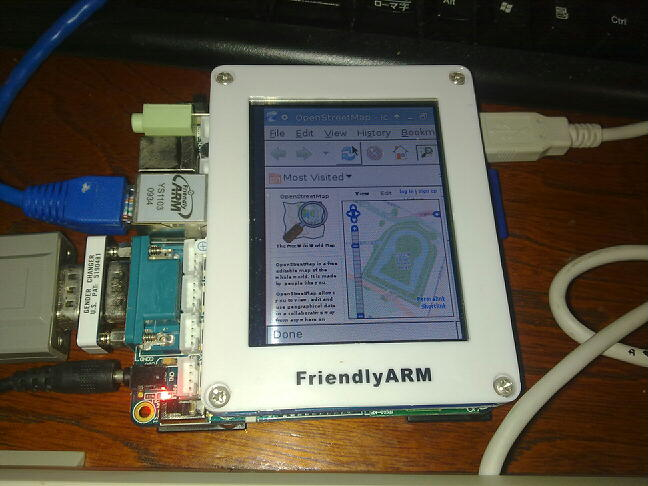
\includegraphics[width=0.8\hsize]{image201008/emdebian.jpg}
\end{center}

MINI2440の詳しい情報は、\url{http://www.friendlyarm.net/products/mini2440}を参照してください。

\subsubsection{必要なもの}

まず、MINI2440のNANDフラッシュROMのバックアップを取るには、残念ながら
MS-Windows上で動くソフトウェア(DNW)が必要です。筆者は、NANDフラッシュROM
のバックアップと、ブートローダ(U-Boot)書き込みに(不本意ですが)MS-Windows
を使いました。(後すみません、TeraTermも使いました)

他に必要なものを以下に記します。
\begin{itemize}
 \item MINI2440本体
 \item i386(amd64)な Debian
 \item ネットワーク
 \item シリアルケーブル(クロスケーブル)
 \item SDカード(1GByte~2GByte)(Debian PCからアクセスするので、カードアダプタも必要)
\end{itemize}

\subsubsection{MINI2440のEmdebian化}

\subsubsubsection{MINI2440 NAND フラッシュのバックアップ(必要なら)}

MINI2440は、購入した状態ではNANDフラッシュROM にQt/Embeddedがインストール
されていますので、もし必要ならばバックアップしてください。

\subsubsubsection{Emdebian Grip rootfs の取得}

\url{http://code.google.com/p/mini2440/wiki/Emdebian}を参考に、Emdebian
Gripのrootfsを取得します。ここではdebootstrapを使いますので、適宜
apt-get等でインストールしておいてください。

Emdebian Grip rootfs は、上記URLに記載している手順で進められます…が、こ
のURLでは、Emdebian Grip向けLinuxカーネルビルドに関する事が無いので、
Emdebian Grip向けのLinuxカーネルをビルドする必要があります。

\subsubsubsection{MINI2440(Emdebian Grip)向けLinuxカーネルのビルド}

MINI2440(Emdebian Grip)向けLinuxカーネルをビルドするには、最低限下記のも
のが必要です。

\begin{enumerate}
 \item Toolchain(gcc)
 \item (MINI2440に対応した)Linux カーネルソース
\end{enumerate}

できれば、それこそEmdebianで一撃に…と思ったのですが、筆者は
\url{http://code.google.com/p/mini2440/downloads/list}から得られる
mini2440-bootstrap-v2.shと言うシェルスクリプトを改造して使いました。

このシェルスクリプト(mini2440-bootstrap-v2.sh)は、開発環境(CodeSoucery)や
MINI2440向けLinuxカーネルを自動的にダウンロードしてビルドします。

なお、mini2440-bootstrap-v2.shは、Debian上でも使えますが、U-Bootのソース
コードはダウンロードしますがビルドはしないので、下記の様に修正して使いま
す。

\begin{commandline}
 tosihisa@lavie:~/Downloads$ diff -ca mini2440-bootstrap-v2.sh mini2440-bootstrap-v2.sh.change
 *** mini2440-bootstrap-v2.sh    2010-08-17 17:19:45.000000000 +0900
 --- mini2440-bootstrap-v2.sh.change     2010-08-17 17:19:13.000000000 +0900
 ***************
 *** 72,78 ****
  # compile bits
  cd ${DEST}/uboot/mini2440
  make mini2440_config
 ! # make clean all

  cd ${DEST}/kernel/mini2440

 --- 72,78 ----
  # compile bits
  cd ${DEST}/uboot/mini2440
  make mini2440_config
 ! make clean all

  cd ${DEST}/kernel/mini2440

 tosihisa@lavie:~/Downloads$
\end{commandline}

\subsubsubsection{U-BootをMINI2440にインストールする。}

MINI2440は、Superviviと言うブートローダがNORフラッシュ側にありますが、
NANDフラッシュ側にU-Bootをインストールします。

U-Boot(the Universal Boot Loader)は、Linux カーネルだけでなく、ELF形式で
あればロードできるブートローダです。また、ブートローダとしての機能だけで
はなく、メモリ操作が可能なので、デバッグツールとしても利用できます。

U-Bootは、\url{http://www.friendlyarm.net/downloads}から入手できるビルド
済みのバイナリ(u-boot\_20100701.zip)を使いました。

\subsubsubsection{Emdebian Grip を起動…}

rootfsを作り、Linux カーネルをビルドできたら、それらをSDカードにコピーし
ます。
U-BootをMINI2440に焼きこめたら、Linuxを起動します。

debootstrap 直後のSDカードで起動した場合、完全にはインストールが完了して
いませんので、U-Bootのブートパラメータに'init=/bin/sh'を与えて、シェルを
起動させるようにします。

その後、(MINI2440で起動したEmdebianで)シェルが起動したら、ネットワークが
DHCPで割り振られた状態で、下記のコマンドを実行する事でEmdebianのインストー
ルが継続されます。

\begin{commandline}
 sh-3.2# /debootstrap/debootstrap --second-stage
\end{commandline}

これが終われば、Emdebian Gripが楽しめます。apt-getでソフトを入れてみてく
ださい。

\subsection{出来てないことだらけ(今後の勉強課題)}
\begin{itemize}
 \item Toolchain も Emdebian のものを使う。
 \item Linux カーネルも Emdebian 由来のものを使ってみたい。
 \item Emdebian Crush を試す。
 \item U-Boot はソースからビルドして使う。
 \item この資料を充実させる(年末には…)
\end{itemize}

\dancersection{今後の予定}{Debian JP}

\subsection{次回の関西Debian勉強会}
次回、2010年9月の関西Debian勉強会は、9月26日(日)に京都の(財)京都高度技術
研究所(ASTEM)8階のコミュニケーションルームをお借りして実施する予定です。

いつもの大阪福島区民センターとは違う場所での開催ですので、事前のアナウン
スにご注意ください。

ネタはまだ決まっていませんが、ネットワークが使えたりして、いつもと違うこ
とができるので、みなさまの発表をお待ちしています。

\subsection{関西オープンソース2010+関西コミュニティ大決戦に参加します}
まだ少し先の話ですが、11月5日(金)と6日(土)に大阪南港ATCにて関西オープンソー
ス2010が開催されます。
8月23日に申し込みが始まりますが、関西Debian勉強会も参加の申し込みをする予
定です。


% 冊子にするために、4の倍数にする必要がある。
% そのための調整

\printindex
 \cleartooddpage

 \begin{minipage}[b]{0.2\hsize}
  \rotatebox{90}{\fontsize{80}{80} {\gt 関西 Debian 勉強会} }
 \end{minipage}
 \begin{minipage}[b]{0.8\hsize}

 \vspace*{15cm}
 \rule{\hsize}{1mm}
 \vspace{2mm}
 
\includegraphics[width=2cm]{image200502/openlogo-nd.eps}
 \noindent \Large \bf Debian 勉強会資料\\ \\
 \noindent \normalfont \debmtgyear{}年\debmtgmonth{}月\debmtgdate{}日 \hspace{5mm}  初版第1刷発行\\
 \noindent \normalfont 関西 Debian 勉強会 (編集・印刷・発行)\\
 \rule{\hsize}{1mm}
 \end{minipage}

\end{document}
